\documentclass[10pt,twocolumn,letterpaper]{article}

\usepackage{cvpr}
\usepackage{times}
\usepackage{epsfig}
\usepackage{graphicx}
\usepackage{amsmath}
\usepackage{amssymb}
%\usepackage{amsfonts}

% Include other packages here, before hyperref.

% If you comment hyperref and then uncomment it, you should delete
% egpaper.aux before re-running latex.  (Or just hit 'q' on the first latex
% run, let it finish, and you should be clear).
\usepackage[breaklinks=true,bookmarks=false]{hyperref}

\cvprfinalcopy % *** Uncomment this line for the final submission

\def\cvprPaperID{****} % *** Enter the CVPR Paper ID here
\def\httilde{\mbox{\tt\raisebox{-.5ex}{\symbol{126}}}}

% Pages are numbered in submission mode, and unnumbered in camera-ready
%\ifcvprfinal\pagestyle{empty}\fi
\setcounter{page}{1}
\begin{document}

%%%%%%%%% TITLE
\title{Dynamic Routing Between Capsules}

\author{Avinash Kommineni\\
University at Buffalo\\
%Institution1 address\\
\href{mailto:akommine@buffalo.edu}{\tt\small akommine@buffalo.edu}
% For a paper whose authors are all at the same institution,
% omit the following lines up until the closing ``}''.
% Additional authors and addresses can be added with ``\and'',
% just like the second author.
% To save space, use either the email address or home page, not both
%\and
%Second Author\\
%Institution2\\
%First line of institution2 address\\
%{\tt\small secondauthor@i2.org}
}

\maketitle
%\thispagestyle{empty}

%%%%%%%%% ABSTRACT
\begin{abstract}
   This project is the understanding and implementation of the algorithm mentioned by \href{mailto:geoffhinton@google.com}{Geoffrey E. Hinton}, the godfather of deep learning in his paper called 'Dynamic Routing Between Capsules'.
\end{abstract}

%%%%%%%%% BODY TEXT
\section{Introduction}

The conventional algorithms being used for image classification such as the Convolutional Neural Networks (CNNs) use translated replicas of learned feature detectors and this allows them to translate knowledge about good weight values acquired at one position in an image to other positions. CNNs have proved to be really good at this job of image recognition but they have got an intrinsic short coming since their inception such as rotation if all the trained images are in a particular rotation, pooling gives some translational invariance in much deeper layers but only in a crude way whereas the human brain must achieve translational invariance in a much better way. Human vision ignores irrelevant details by using a carefully determined sequence of fixation points to ensure that only a tiny fraction of the optic array is ever processed at the highest resolution. 

Geoffrey E. Hinton coined the term capsule in 2011 paper `Transforming Auto-encoders' as local pool of neurons that perform some quite complicated internal computations on their inputs and then encapsulate the results of these computations into a small vector of highly informative outputs. A capsule is a group of neurons whose activity vector represents the instantiation parameters of a specific type of entity such as an object or object part. We use the length of the activity vector to represent the probability that the entity exists and its orientation to represent the instantiation parameters. Active capsules at one level make predictions, via transformation matrices, for the instantiation parameters of higher-level capsules.

This algorithm though in its budding state has created waves across the deep learning community for its unique way of thought and its potential growth. By this project I would have the opportunity of studying and understanding closely what are the recent advancements of the research community.


%-------------------------------------------------------------------------


\section{Related Work}
This project is completely based of the recent publication, `Dynamic Routing Between Capsules'\cite{dynamicRouting} though the idea of capsules has been for a while and other state-of-the-art performing algorithms based on CNN from several communities like Alexnet, VGGNet, GoogleNet, ResNet, DenseNet are all aimed for bigger problems with higher dimensions.

\section{Algorithm}
Since Human vision ignores irrelevant details by using a carefully determined sequence of fixation points, in this paper we will assume that a single fixation gives us much more than just a single identified object and its properties. We will assume that our multi-layer visual system creates something like a parse tree on each fixation, and we will ignore the issue of how these single-fixation parse trees are coordinated over multiple fixations. Each layer will be divided into many small groups of neurons called capsules and each node in the parse tree will correspond to an active capsule. Using an iterative routing process, each active capsule will choose a capsule in the layer above to be its parent in the tree.\\

The activities of the neurons within an active capsule represent the various properties of a particular entity that is present in the image. These properties can include many different types of instantiation parameter such as pose (position, size, orientation), deformation, velocity, albedo, hue, texture etc. One very special property is the existence of the instantiated entity in the image. An obvious way to represent existence is by using a separate logistic unit whose output is the probability that the entity exists. The paper explores an interesting alternative which is to use the overall length of the vector of instantiation parameters to represent the existence of the entity and to force the orientation of the vector to represent the properties of the entity. It has also been made sure that the length of the vector output of a capsule cannot exceed 1 by applying a non-linearity that leaves the orientation of the vector unchanged but scales down its magnitude.\\

The fact that the output of a capsule is a vector makes it possible to use a powerful dynamic routing mechanism to ensure that the output of the capsule gets sent to an appropriate parent in the layer above. Initially, the output is routed to all possible parents but is scaled down by coupling coefficients that sum to 1. For each possible parent, the capsule computes a “prediction vector” by multiplying its own output by a weight matrix. If this prediction vector has a large scalar product with the output of a possible parent, there is top-down feedback which has the effect of increasing the coupling coefficient for that parent and decreasing it for other parents. This increases the contribution that the capsule makes to that parent thus further increasing the scalar product of the capsule’s prediction with the parent’s output.\\

Convolutional neural networks (CNNs) use translated replicas of learned feature detectors and this allows them to translate knowledge about good weight values acquired at one position in an image to other positions. This has proven extremely helpful in image interpretation. Even though we are replacing the scalar-output feature detectors of CNNs with vector-output capsules and max-pooling with routing-by-agreement, we would still like to replicate learned knowledge across space, so we make all but the last layer of capsules be convolutional. As with CNNs, we make higher-level capsules cover larger regions of the image, but unlike max-pooling we do not throw away information about the precise position of the entity within the region. For low level capsules, location information is “place-coded” by which capsule is active. As we ascend the hierarchy more and more of the positional information is “rate-coded” in the real-valued components of the output vector of a capsule. This shift from place-coding to rate-coding combined with the fact that higher-level capsules represent more complex entities with more degrees of freedom suggests that the dimensionality of capsules should increase as we ascend the hierarchy.
In CNNs, the max-pooling allows neurons in one layer to ignore all but the most active feature detector in a local pool in the layer below. So a new type of routing-by-agreement mechanism: A lower-level capsule prefers to send its output to higher level capsules whose activity vectors have a big scalar product with the prediction coming from the lower-level capsule.

\section{Implementation}
\subsection{Squashing}
The length of output vector of a capsule represents the probability that the entity represented by the capsule is present in the current input. A non-linear `squashing' function is used to ensure that short vectors get shrunk to almost zero length and long vectors get shrunk to a length slightly below 1.
\[ \hat{u’}_{j|i} = W_{ij}u_i \]
\[ s_j = \sum_j c_{ij} \hat{u’}_{j|i} \]
 where $c_{ij}$ are coupling coefficients that are determined by the iterative dynamic routing process.
\[ v_j = \frac{||s_j||^2}{1+||s_j||^2}\frac{s_j}{||s_j||}\]

The coupling coefficients between capsule i and all the capsules in the layer above sum to 1 and are determined by a `routing softmax' whose initial logits bij are the log prior probabilities that capsule i should be coupled to capsule j.
\[ c_{ij} = \frac{exp(b_{ij})}{\sum_k exp(b_{ik})} \]
The log priors can be learned discriminatively at the same time as all the other weights. They depend on the location and type of the two capsules but not on the current input image.

\subsection{Routing}
\begin{figure*}[ht]
	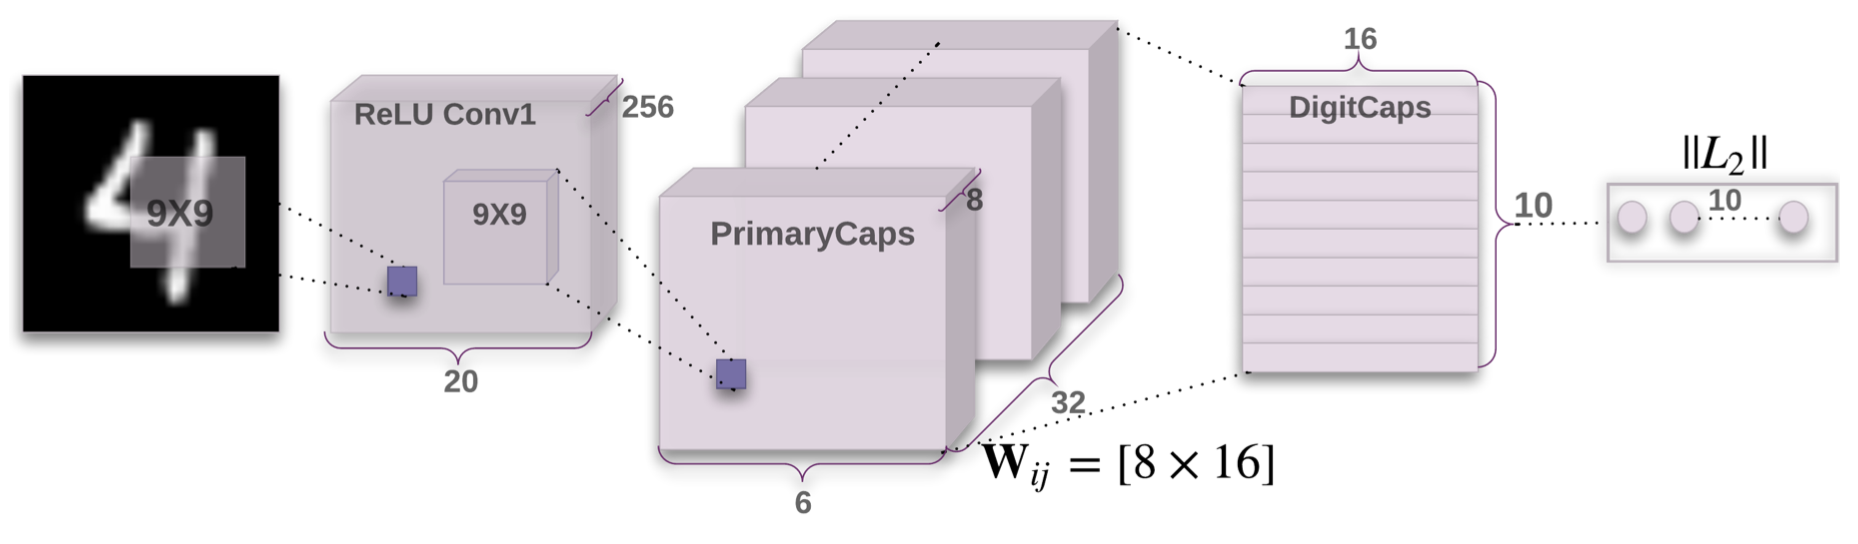
\includegraphics[width=\textwidth]{1}
	\caption{CapsNet Architecture}
\end{figure*}
Capsule routing consists of the following steps...
\begin{enumerate}
	\item for all capsule $i$ in layer $l$ and capsule $j$ in layer $(l + 1)$: $b_{ij} \leftarrow 0$.
	\item for n iterations...
	\begin{enumerate}
		\item for all capsule $i$ in layer $l$: $c_i \leftarrow$ $softmax(b_i)$
		\item for all capsule $j$ in layer $(l + 1)$: $s_j \leftarrow \sum_i c_{ij} \hat{u’}_{j|i}$
		\item for all capsule $j$ in layer $(l + 1): v_j \leftarrow squash(s_j)$
		\item for all capsule $i$ in layer $l$ and capsule $j$ in layer $(l + 1): b_{ij} \leftarrow b_{ij} + \hat{u’}_{j|i}.v_j$
	\end{enumerate}
\end{enumerate}

\subsection{Loss Function}
Since the length of instantiation vector represents the probability that a capsule’s entity exists, the top-level capsule for digit class $k$ to have a long instantiation vector if and only if that digit is present in the image. To allow for multiple digits, a separate margin loss, $L_k$ for each digit capsule, $k$:
\[ L_c = T_c max(0,m^+ - ||V_c||)^2 + \lambda(1-T_c)max(0,||V_c|| - m^-)^2 \]

where $T_c = 1$ if a digit of class c is present in the image and $m^+ = 0.9$ and $m^- = 0.1$. The $\lambda$ down-weighting of the loss for absent digit classes stops the initial learning from shrinking the lengths of the activity vectors of all the digit capsules. As suggested by the paper $\lambda = 0.5$ is used.

\subsection{CapsNet Architecture}
The architecture is shallow with only two convolutional layers and one fully connected layer. Conv1 has 256, 9 × 9 convolution kernels with a stride of 1 and ReLU activation. This layer converts pixel intensities to the activities of local feature detectors that are then used as inputs to the primary capsules.\\
The second layer (PrimaryCapsules) is a convolutional capsule layer with 32 channels of convolutional 8D capsules (i.e. each primary capsule contains 8 convolutional units with a 9 x 9 kernel and a stride of 2). Each primary capsule output sees the outputs of all 256 x 81 Conv1 units whose receptive fields overlap with the location of the center of the capsule. In total PrimaryCapsules has [32, 6, 6] capsule outputs (each output is an 8D vector) and each capsule in the [6, 6] grid is sharing their weights with each other. One can see PrimaryCapsules as a Convolution layer as its block non-linearity. The final Layer (DigitCaps) has one 16D capsule per digit class and each of these capsules receives input from all the capsules in the layer below.
We have routing only between two consecutive capsule layers (e.g. PrimaryCapsules and DigitCaps). Since Conv1 output is 1D there is no orientation in its space to agree on. Therefore, no routing is used between Conv1 and PrimaryCapsules. All the routing logits $(b_{ij})$ are initialized to zero. Therefore, initially a capsule output $(u_i)$ is sent to all parent capsules $(v_0 ...v_{10})$ with equal probability $(c_{ij})$.

\subsubsection{Reconstruction as a regularization method}
\begin{figure}[ht]
	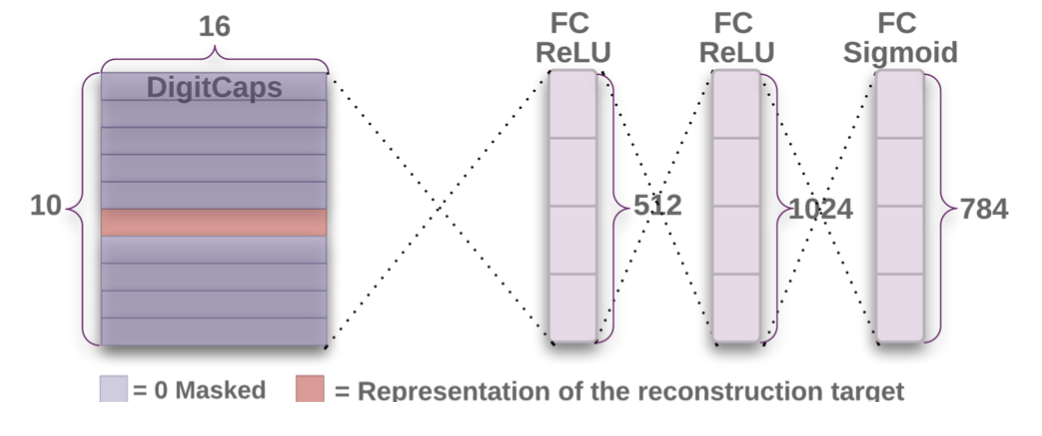
\includegraphics[width=\columnwidth]{2}
	\caption{Reconstruction}
\end{figure}
Reconstruction loss is used to encourage the digit capsules to encode the instantiation parameters of the input digit. In contains of 2 fully connected layers with ReLU activation and then to 784 with sigmoid so that they can be mapped to 28x28 pixel image (same as the input). Only the activity vector corresponding to the correct digit capsule is fed into the network. Reconstruction error can be defined as the squared differences between the outputs of the logistic units and the pixel intensities. Reconstruction loss is scaled down by 0.0005 so that it does not dominate the margin loss during training.

\section{Results and Observations}
An accuracy of 99.4\% is acheived on the MNIST dataset with 10 epochs.\\
The paper mentions an accuracy of 99.75\% accuracy which cannot be be acheived by conventional shallow CNNs. Only acheived by deep networks.\\
This idea is still in the development stage but the other interesting observations are as follows...
\begin{enumerate}
	\item Dynamic routing can be viewed as a parallel attention mechanism that allows each capsule at one level to attend to some active capsules at the level below and to ignore others. Consider the example of a rectangle and a traingle, both in a particular orientation (wrt each other) only contribute to form a boat but the same can also be used to make a house. The conventional CNNs have detectors for both these and shape and thus output `True' for both thses classes unlike Capsule Networks which takes into account of relative sizes and orientation.
	\item Each dimension in the final DigitCaps contribute to some information regarding the image like stroke thickness, skew and width. 
	\item They also include digit-specific variations such as the length of the tail of a 2.
	\item The individual dimensions contribution can be known by using of the decoder network.
	\item Because of its network configuration, the model is robust to small affine transformations.
\end{enumerate}
\begin{figure}[ht]
	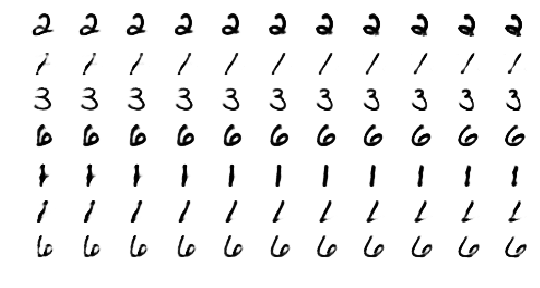
\includegraphics[width=\columnwidth]{j0}
	\caption{Tweaking output dimension \#0}
\end{figure}
\begin{figure}[ht]
	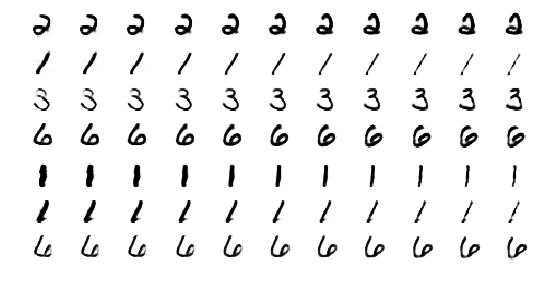
\includegraphics[width=\columnwidth]{j1}
	\caption{Tweaking output dimension \#1}
\end{figure}
\begin{figure}[ht]
	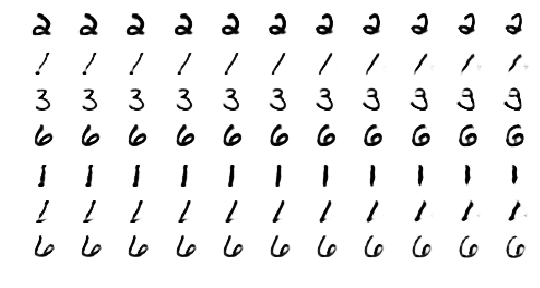
\includegraphics[width=\columnwidth]{j2}
	\caption{Tweaking output dimension \#2}
\end{figure}
\begin{figure}[ht]
	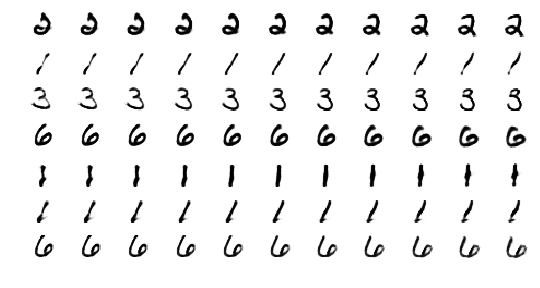
\includegraphics[width=\columnwidth]{j3}
	\caption{Tweaking output dimension \#3}
\end{figure}
\begin{figure}[ht]
	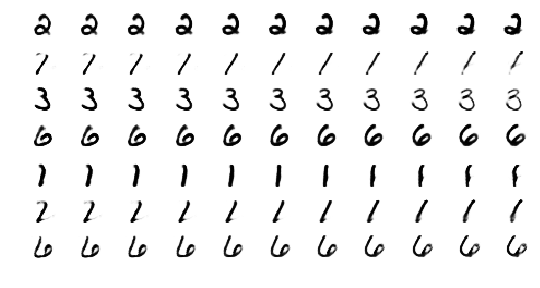
\includegraphics[width=\columnwidth]{j4}
	\caption{Tweaking output dimension \#4}
\end{figure}
\begin{figure}[ht]
	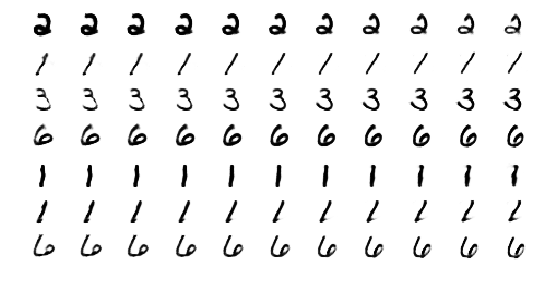
\includegraphics[width=\columnwidth]{j5}
	\caption{Tweaking output dimension \#5}
\end{figure}
\begin{figure}[ht]
	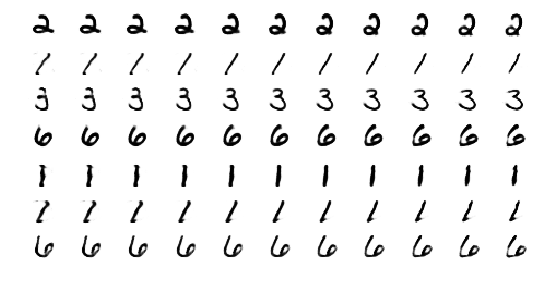
\includegraphics[width=\columnwidth]{j6}
	\caption{Tweaking output dimension \#6}
\end{figure}
\begin{figure}[ht]
	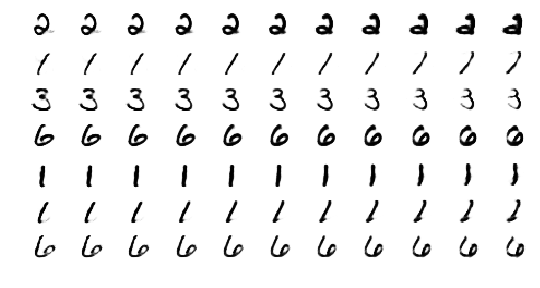
\includegraphics[width=\columnwidth]{j7}
	\caption{Tweaking output dimension \#7}
\end{figure}
\begin{figure}[ht]
	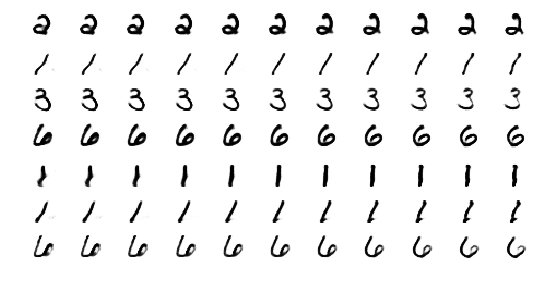
\includegraphics[width=\columnwidth]{j8}
	\caption{Tweaking output dimension \#8}
\end{figure}
\begin{figure}[ht]
	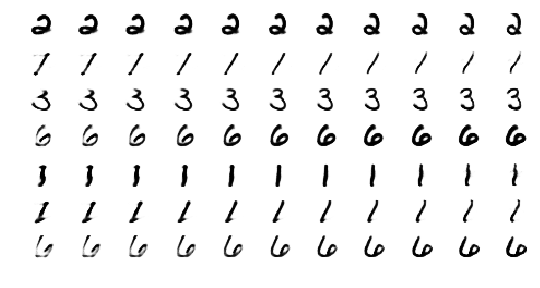
\includegraphics[width=\columnwidth]{j9}
	\caption{Tweaking output dimension \#9}
\end{figure}
\begin{figure}[ht]
	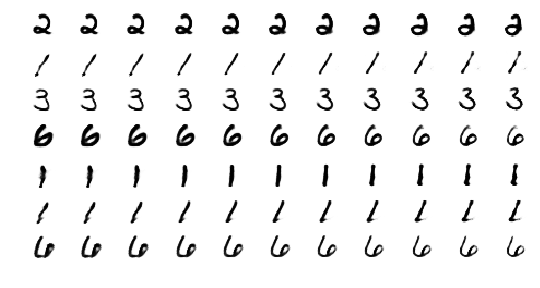
\includegraphics[width=\columnwidth]{j10}
	\caption{Tweaking output dimension \#10}
\end{figure}
\begin{figure}[ht]
	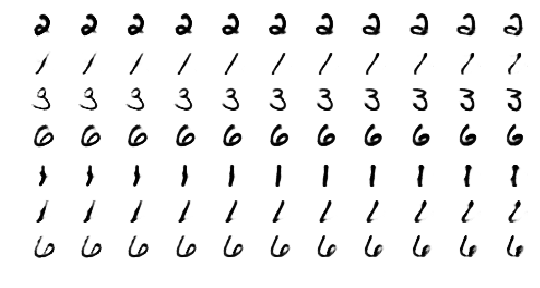
\includegraphics[width=\columnwidth]{j11}
	\caption{Tweaking output dimension \#12}
\end{figure}
\begin{figure}[ht]
	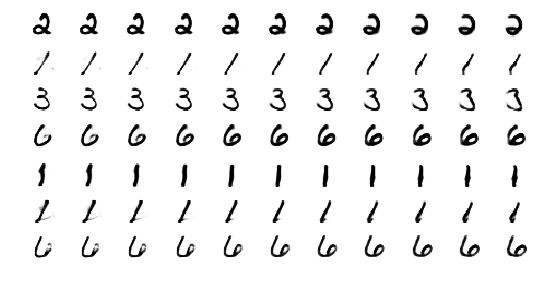
\includegraphics[width=\columnwidth]{j12}
	\caption{Tweaking output dimension \#12}
\end{figure}
\begin{figure}[ht]
	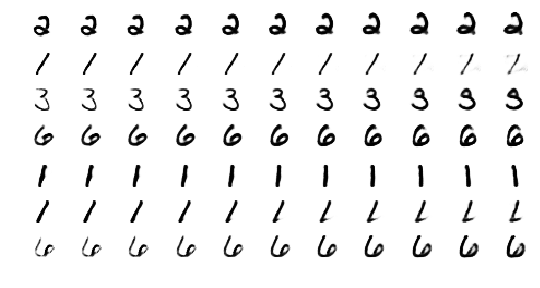
\includegraphics[width=\columnwidth]{j13}
	\caption{Tweaking output dimension \#13}
\end{figure}
\begin{figure}[ht]
	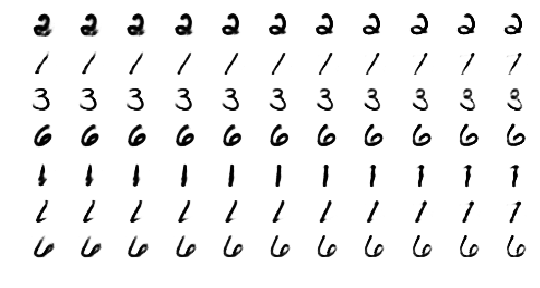
\includegraphics[width=\columnwidth]{j14}
	\caption{Tweaking output dimension \#14}
\end{figure}
\begin{figure}[ht]
	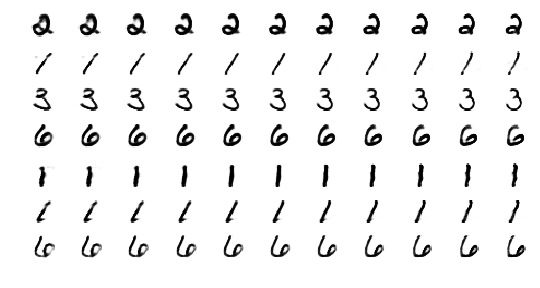
\includegraphics[width=\columnwidth]{j15}
	\caption{Tweaking output dimension \#15}
\end{figure}

\vfill
\begin{thebibliography}{9}
	\bibitem{dynamicRouting} 
	Sara Sabour, Nicholas Frosst, Geoffrey E. Hinton
	\textit{Dynamic Routing Between Capsules}. 
	Computer Vision and Pattern Recognition, 2017.
\end{thebibliography}

\end{document}
